% Primarily this section should be about scientific methods and theories you need to evaluate/compare/invent to solve your problems from 1.3.
% In some cases it may be ok to describe different technologies, but the purpose is to describe something and then draw a conclusion from that.
% Example, if you decide to discuss different databases, it may be for the purpose of selecting the best type for your implementation later on (based on for example data representation, scalability, speed, etc.).
% Optimally the problems in 1.3 are not solved by anyone else yet, in which case this section needs to describe how to solve them (new algorithms, mathematical approaches, etc.).
 
% This section can have a lot of subsections (3.1, 3.2, 3.3, etc).

% TODO: Explain DWARF Die

One of the most important data structures in the \gls{DWARF} format is the \gls{die} which are found in the \emph{.debug\_info} and \emph{.debug\_type} sections.
These \glspl{die} are used to represent parts of the source code and hold information about were in the source code there are declared.
They also contain information about which range of addresses they are applicable to in the machine code and more.
There are two types of \glspl{die}, one of them are dies that only describe types in the source code and are located in a \gls{tree} in the section \emph{.debug\_types}.
The other type of \gls{die} are dies that describe the structure of the source code and describes where that information is in the machine code.


Let look at an example of a \gls{die} that describes a variable, the example can be seen in figure \ref{fig:dwarfdie} which is a screen shoot of the output from the program \emph{objdump} run on a \gls{elf} file.
The first line in the figure begins with a number $8$ which represents the depth in the tree this \gls{die} is located, the next number is the offset into this section for that line.
Lastly the information stored on that line is a $9$ which represents the tag of the \gls{die} which is in this case \emph{DW\_AT\_variable}.
This first line is also the first line of the die.
For the rest of the line the first number is also the offset into the \emph{.debug\_info} section that the information is located and these lines are attributes to in the \gls{die}.
The attribute \emph{DW\_AT\_location} has the information of where the variable is stored on the \gls{debugee}.
The name attribute \emph{DW\_AT\_name} has an offset into the \gls{DWARF} section \emph{.debug\_str} that the tool has evaluated to "str" and it is the name of the variable.
The attributes \emph{DW\_AT\_decl\_file} and \emph{DW\_AT\_decl\_line} has offset into the section \emph{.debug\_line} and will reveal the source file and line that this \gls{die} comes from.
Lastly the attribute \emph{DW\_AT\_type} has a offset into the section \emph{.debug\_types} that points to a type \gls{die} that has the type information for this variable.


\begin{figure}[h]
	\centering
	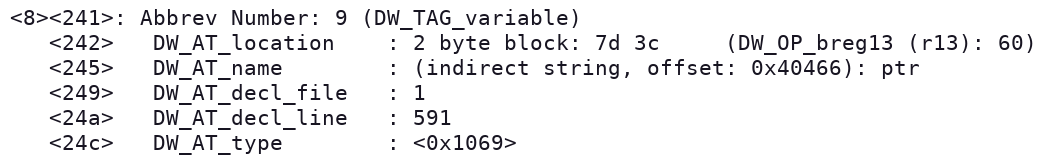
\includegraphics[width=1.0\textwidth]{dwarf-die.png}
	\caption{An example of a \gls{DWARF} \gls{die} for a variable \emph{ptr}. This example is the output of the tool \emph{objdump} run on a \gls{DWARF} file.}
	\label{fig:dwarfdie}
\end{figure}

